
\section{Terms and Related Data Structures}
\label{sec:terms}

The TERMS library provides data types and functions realizing an
efficient term representation. It includes both conventional terms and
banks of maximally shared terms with efficient indexing and paralell
rewriting of shared terms.

\subsection{Function Symbols and Variables}
\label{sec:terms:sigs}

Function symbols and variable symbols are internally represented by
the data type \texttt{FunCode} (currently realised as an alias for C
long integers). Positive values are used to represent function
symbols, negative values represent variable symbols. Information about
how to interpret this values for a given set of terms are collected in
\texttt{SigCell} structures (storing the information usually given in
a \emph{signature}) and \texttt{VarTransCell} structures.

\subsubsection{Usage Information}

\begin{verbatim}
#include <cte_signature.h>
#include <cte_termvars.h>

Requires: lib/BASICS.a
          lib/INOUT.a
          lib/TERMS.a
\end{verbatim}


\subsubsection{Signatures}
\label{sec:terms:sigs:sigs}

A \texttt{SigCell} structure stores information about external and
internal representation of function symbols. Knowledge about the
internal organisation of this data structure should be unnecessary,
all necessary operations are supported via the following interface
functions: 

\begin{verbatim}
Sig_p SigAlloc()
\end{verbatim}
\begin{quote}
  Allocate and initialize a \texttt{SigCell}. This funtion always
  inserts the special function symbol \verb-$bottom- with the \texttt{FunCode}
  \texttt{SIG\_BOTTOM\_CODE} and arity 0. If the variable
  \texttt{SigSupportsList} has the value \texttt{true}, the newly
  allocated signature will also contain the symbols \verb-$nil- with
  arity 0 and \texttt{FunCode} \texttt{SIG\_NIL\_CODE}, and \verb-$cons- with
  arity 2 and \texttt{FunCode} \texttt{SIG\_CONS\_CODE}, which are used to
  represent PROLOG lists as normal terms.
\end{quote}


\begin{verbatim}
void SigFree(Sig_p junk)
\end{verbatim}
\begin{quote}
  Return the memory used by a signature to the memory mangament.
\end{quote}

\begin{verbatim}
FunCode SigFindFCode(Sig_p sig, char* name)
\end{verbatim}
\begin{quote}
  Return the \texttt{FunCode} value for a symbol with the given name.
\end{quote}

\begin{verbatim}
int SigFindArity(Sig_p sig, FunCode f_code)
\end{verbatim}
\begin{quote}
  Return the arity of the function symbol with the given \texttt{FunCode}. 
\end{quote}

  \begin{verbatim}
char* SigFindName(Sig_p sig, FunCode f_code)
\end{verbatim}
\begin{quote}
  Return the external name of the function symbol with the given
  \texttt{FunCode}. The pointer is only valid as long as the signature
  exists. Use SecureStrdup() if you want a permanent copy.
\end{quote}

\begin{verbatim}
FunCode SigInsertId(Sig_p sig, char* name, int arity)
\end{verbatim}
\begin{quote}
  Given an external name and an arity, insert the function symbol into
  the signature (if it is not already stored) and returns its
  \texttt{FunCode}. If the new symbol is incompatible with the
  signature (because it has already been used with another arity)
  return 0.
\end{quote}

\begin{verbatim}
void SigPrint(FILE* out, Sig_p sig)
\end{verbatim}
\begin{quote}
  Print the signature to the given output channel.
\end{quote}


\subsubsection{Variable Banks}
\label{sec:terms:sigs:variables}

CLIB allows variables to be shared in terms, that is a variable with a
given \texttt{FunCode} value will always be represented by the same
term cell in a given term (or set of terms). While it is possible to
construct terms without this property, the normal routines of CLIB
will only construct terms with this property (except for short term
\emph{bindings} which may combine parts from several distinct terms)
and often require this property to work properly.

Variables are managed by \emph{variable banks} (\texttt{VarBankCell}
structures). Varbiable banks maintain an index from a \texttt{Funcode}
value to a term cell, and also translate external variable
representations to internal \texttt{FunCode} values in a consistent
way during parsing.

Most users of the library will need only the allocation and
deallocation functions (or not even those if only fully shared terms
are used - term banks handle variable banks transparently). The other
functions are only necessary if you intend to write your own parsing
routines for term-like objects.

\begin{verbatim}
VarBank_p VarBankAlloc()
\end{verbatim}
\begin{quote}
  Create an initialized \texttt{VarBank} structure and return the
  pointer to it.
\end{quote}

\begin{verbatim}
void VarBankFree(VarBank_p junk)
\end{verbatim}
\begin{quote}
  Free the memory taken by a \texttt{VarBank} structure.
\end{quote}

\begin{verbatim}
void VarBankClearExtNames(VarBank_p bank)
\end{verbatim}
\begin{quote}
  Reset the external name to \texttt{FunCode} mapping. You can call
  this between parsing independend term set to ensure that all terms
  are variable-normalized as far as possible.
\end{quote}

\begin{verbatim}
Term_p VarBankFCodeFind(VarBank_p bank, FunCode f_code)
\end{verbatim}
\begin{quote}
  Return a pointer to the variable with a given \texttt{FunCode} in
  the term bank, \texttt{NULL} if no such variable exists.
\end{quote}

\begin{verbatim}
Term_p VarBankExtNameFind(VarBank_p bank, char* name)
\end{verbatim}
\begin{quote}
  Return a pointer to the variable with a given exterbak name in the
  term bank, \texttt{NULL} if no such variable exists.
\end{quote}

\begin{verbatim}
Term_p VarBankFCodeAssertAlloc(VarBank_p bank, FunCode f_code)
\end{verbatim}
\begin{quote}
  If there is a variable with \texttt{FunCode} \texttt{f\_code} in the
  variable bank, return the pointer to it. Otherwise create such a
  variable in the varbank and return the pointer.
\end{quote}

\begin{verbatim}
Term_p VarBankExtNameAssertAlloc(VarBank_p bank, char* name)
\end{verbatim}
\begin{quote}
  If there is a variable with the given external name in the variable
  bank, return the pointer to it. Otherwise create such a variable in
  the varbank and return the pointer. Note that new \texttt{FunCode}
  values are handed out systematically (from the set $\{-1,
  -2,\ldots\}$). If calls to \texttt{VarBankFCodeAssertAlloc()} and
  \texttt{VarBankExtNameAssertAlloc()} are miced, variables introduced
  by \texttt{VarBankFCodeAssertAlloc()} may be bound to new external
  names.
\end{quote}




\subsection{Unshared Terms}
\label{sec:terms:unshared}

This section describes the structure and implementation of terms as
trees. Most of the data structures and elementary functions for
unshared terms are defined in \texttt{cte\_termtypes.h}, while more
complex functions can be found in  \texttt{cte\_termfuncs.h}.

\subsubsection{Usage Information}

\begin{verbatim}
#include <cte_termfunc.h>

Requires: lib/BASICS.a
          lib/INOUT.a
          lib/TERMS.a
\end{verbatim}

\subsubsection{The \texttt{TermCell} Data Type}

\texttt{TermCell} structures (and the \texttt{Term\_p} pointer type)
are used for the representation of both simple, unshared terms and the
shared term bank data structure introduced in
Sec.~\ref{sec:terms:banks}.  Most of the conventional functionality
of terms is defined for unshared terms and only inherited by the
shared data types, however, there some serious differences for
functions that create side effects or that need to touch each term
cell only once.

A unshared term is basically an ordered tree structure.
Fig~\ref{fig:terms:unshared} shows an example for the internal
representation of an unshared term as realized by the CLIB library.

\begin{figure}[htb]
  \begin{center}
    \mbox{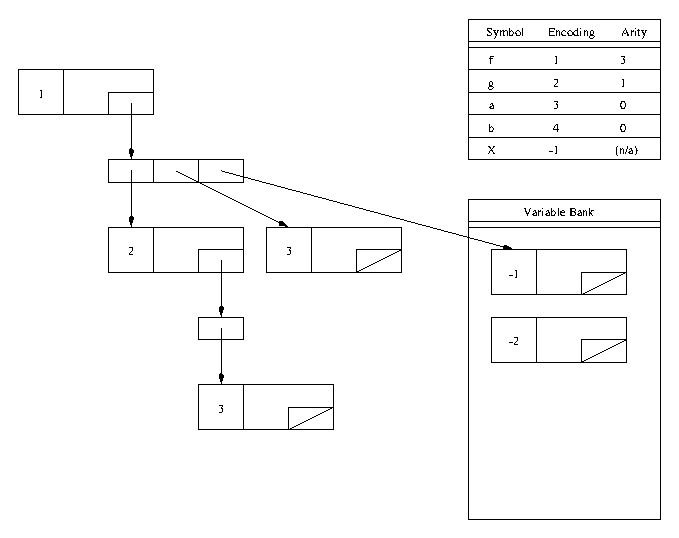
\epsfig{file=unshared_terms.eps}}
    \caption{Representation for the term \texttt{f(g(a),a,X)}}
    \label{fig:terms:unshared}
  \end{center}
\end{figure}

A cell for each term node contains information about the function
symbol, and a pointer to an array of argument terms. It also contains
additional information about the term and slots used only for the
implementation of functionality of shared terms. A term cell is
realized as the following C language \texttt{struct} (only elements
necessary for unshared terms are shown here, see
section~\ref{sec:terms:banks} for a more complete picture):

\small
\begin{verbatim}
typedef struct termcell
{
   TermProperties   flags;   /* Like basic, lhs, top */
   FunCode          f_code;  /* Top symbol of term */
   int              arity;   /* Redundant, but saves handing around
                                the signature all the time */
   struct termcell* *args;   /* Pointer to array of arguments */
   struct termcell* binding; /* For variable bindings, potentially
                                for temporary rewrites */
   ...
}TermCell, *Term_p, **TermRef;
\end{verbatim}
\normalsize

\begin{description}
\item[\textmd{\texttt{flags}}:] Stores special properties for term
  nodes. This feature is discussed in the next section.
\item[\textmd{\texttt{f\_code}}:] The encoded function symbol or
  variable.
\item[\textmd{\texttt{arity}}:] The number of principal subterms of
  this term cell. If this is 0, the \texttt{args} element should
  contain \texttt{NULL}, otherwise it should point to an memory block
  of size \texttt{arity*sizeof(Term\_p)} that is interpreted as an
  array of \texttt{Term\_p} pointers.
\item[\textmd{\texttt{args}}:] Pointer to the array or argumens.
\item[\textmd{\texttt{binding}}:] If this pointer is not
  \texttt{NULL}, it points to another term, that can be used instead
  of the current term cell (and corresponding term). This feature is
  mainly intended for the instantiation of variables, but can also be
  used if you want to modify a term temporarily. Most functions on
  terms can be told to follow or ignore bindings.
\end{description}


\subsubsection{Term Properties}

Term properties are stored in individual bits of the \texttt{flags}
field. The relevant data type, \texttt{TermProperties}, is defined as
an enumeration type in \texttt{cte\_terms.h}\footnote{According to the
  ANSI C standard, enumeration values are compatible with \texttt{int}
  values, i.e. they have at least 32 bits. Thus, 32 distinct
  properties can be assigned to each term.}. Only a few values are
predefined by the library, other values can be defined by the user.

\small
\begin{verbatim}
typedef enum 
{
   TPIgnoreProps = 0, /* For masking properties out */
   TPMaximal     = 1, /* Maximal term == Left hand side */
   TPTopPos      = 2, /* This cell is a entry point */
   TPBasicPos    = 4, /* Basic position on this term */
   TPPredPos     = 8, /* This is an previous predicate position
                         morphed into a term */
   TPOpFlag      = 256,/* For internal use */
   TPOutputFlag  = 512 /* Has this term already been printed? */
}TermProperties;
\end{verbatim}
\normalsize

As properties are bit-valued, they can be combined with the binary
\emph{or}-operator ('\texttt{|}').  Properties are manipulated by
three functions (realised as C preprocessor macros):

\begin{verbatim}
MACRO void TermSetProp(Term_p term, TermProperties prop)
\end{verbatim}
\begin{quote}
  Set the given properties in the term.
\end{quote}

\begin{verbatim}
MACRO void TermDelProp(Term_p term, TermProperties prop)
\end{verbatim}
\begin{quote}
  Delete the given properties in the term.
\end{quote}
\begin{verbatim}
MACRO bool TermQueryProp(Term_p term, TermProperties prop)
\end{verbatim}
\begin{quote}
  Query the given properties. The result is true if all the queried
  properties are set in the term.
\end{quote}


\subsection{Term Banks}
\label{sec:terms:banks}

Term banks are structures for building shared terms. 




%%% Local Variables: 
%%% mode: latex
%%% TeX-master: "clib"
%%% End: 
